\documentclass[12pt, a4paper]{article}

\usepackage[utf8]{inputenc} % кодировка
\usepackage[english, russian]{babel} % Система переносов
\usepackage[T2A]{fontenc} % font encoding
\usepackage{tempora} % шрифт Tempora (Tempora-TLF)

\usepackage[pdftex]{graphicx} % images

% mathematical formulas
\usepackage{amssymb}
\usepackage{amsmath}
\usepackage{geometry}
\usepackage{amsfonts} % подкл. дополнительных мат. шрифтов
\usepackage{latexsym} % некоторые редкие символыs

\usepackage{indentfirst} % отступ в первом абзаце

\usepackage{listings} % code
\usepackage{fancyhdr}
\usepackage{float}
\usepackage{url}
\usepackage{cite} % ссылки на литературу в виде [1-5,9]

% добавить точку после номера раздела
\renewcommand{\thesection}{\arabic{section}.}
\renewcommand{\thesubsection}{\thesection\arabic{subsection}.}
\renewcommand{\thesubsubsection}{\thesubsection\arabic{subsubsection}.}

%Точка вместо двоеточия после номеров рисункоа и таблиц
\usepackage{caption2} 
\renewcommand{\captionlabeldelim}{.}

\title
{
	Равномерное распределение точек на сфере
}
\author
{
	И.Б.Рахимов\thanks{Автор оригинальной статии Мартин Робертс} \\
	студент 2-го курса Магистратуры  \\
	кафедры Вычислительной математики и \\
	прикладных информационных технологий \\
	факультета Прикладной математики, информатики и механики \\
	Воронежского Государственного Университета
}
\date
{
	\today
}

\begin{document}

\maketitle
\thispagestyle{empty} % удаление нумерации на 1-ой странице

\newpage

\begin{abstract}
Как можно более равномерное распределение точек на сфере — невероятно важная задача в математике, науке и компьютерных системах, а наложение сетки Фибоначчи на поверхность сферы при помощи равновеликой проекции — чрезвычайно быстрый и эффективный метод аппроксимации для её решения. В данной работе будет показано, как благодаря незначительным изменениям его можно сделать ещё лучше.
\end{abstract}

\newpage

\tableofcontents

\addcontentsline{toc}{section}{Аннотация} % toc - table of contents

\newpage

\section*{Введение}
\addcontentsline{toc}{section}{Введение} % toc - table of contents

Задача равномерного распределения точек на сфере имеет очень долгую историю. Это одна из самых хорошо исследованных задач в математической литературе по сферической геометрии. Она имеет критическую важность во многих областях математики, физики, химии, в том числе в вычислительных методах, теории приближений, теории кодирования, кристаллографии, электростатике, компьютерной графике, морфологии вирусов и многих других.

К сожалению, за исключением нескольких особых случаев (а именно платоновых тел) невозможно идеально ровно распределить точки на сфере. Кроме того, решение задачи сильно зависит от критерия, который используется для оценки однородности. На практике используется множество критериев, в том числе:

\begin{itemize}
	\item Упаковка и покрытие \cite{alaxandrow_2009};
	\item Выпуклые оболочки, ячейки Вороного и треугольники Делоне \cite{alaxandrow_2009, berg_2016};
	\item Ядра $s$-энергии Риса \cite{alaxandrow_2009, berg_2016, demidovich_2019};
	\item Кубатура и определители \cite{alaxandrow_2009, demidovich_2019}.
\end{itemize}

Очень важно уяснить этот аспект: обычно не существует единственного оптимального решения этой задачи, потому что оптимальное решение, основанное на одном критерии, часто не является оптимальным распределением точек для других. Например, мы также выясним, что оптимизация упаковки необязательно создаёт оптимальную выпуклую оболочку и наоборот.

Ради краткости в этой статье мы рассмотрим только два критерия: минимальное расстояние упаковки и выпуклую оболочку/сетку Делоне (объём и площадь).

В разделе 1 мы покажем, как можно изменить каноническую сетку Фибоначчи для построения улучшенного распределения упаковки. В разделе 2 мы покажем, как можно изменить каноническую сетку Фибоначчи для построения улучшенных параметров выпуклых оболочек (объёма и площади поверхности).

\newpage

\section{Оптимизация расстояния упаковки}

Часто эту задачу называют задачей Тэммса в честь ботаника Тэммса, искавшего объяснение структуры поверхности пыльцевых зёрен. Критерий упаковки требует от нас максимизировать наименьшее расстояние между соседями для $N$ точек. То есть:

\begin{displaymath}
	d_N = \min_{i \neq j} \Vert x_i - x_j \Vert _2,
\end{displaymath}

\noindent это значение уменьшается со скоростью $\dfrac{1}{\sqrt{N}}$, поэтому полезно будет определить нормализованное расстояние, а также асимптотический предел нормализованного расстояния как:

\begin{displaymath}
	d^*_N = \sqrt{N} d_N,
	\qquad
	d^* = \lim_{N \rightarrow \infty} d^*_N.
\end{displaymath}

\subsection{Сетка Фибоначчи}

Одно очень элегантное решение моделирует узлы, встречающиеся в природе, это явление называется спиральным филлотаксисом. Коксетер показал, что такие структуры имеют фундаментальную связь с рядом Фибоначчи:

\begin{displaymath}
	F_k = \{1, 1, 2, 3, 5, 8, 13, \ldots \}
\end{displaymath}

\noindent и золотым сечением:

\begin{displaymath}
	\phi = \frac{1 + \sqrt{5}}{2}.
\end{displaymath}

В литературе встречается два схожих определения множества точек сферической сетки Фибоначчи. Исходное определено строго для $N$, равного одному из членов ряда Фибоначчи, $F_m$, и хорошо изучено в теории чисел:

\begin{displaymath}
	t_i = \left( \frac{i}{F_m}, \frac{i \cdot F_{m-1}}{F_m} \right),
	\qquad
	0 \leq i \leq N-1.
\end{displaymath}

Второе определение, при котором $d^* = 2$, обобщает формулу до произвольного количества $N$ и используется в вычислениях чаще:

\begin{displaymath}
	t_i = \left( \frac{i}{N}, \frac{i}{\phi} \right),
	\qquad
	0 \leq i \leq N-1,
	\tag{1}
\end{displaymath}

\begin{displaymath}
	\phi = \frac{1 + \sqrt{5}}{2} = \lim_{n \rightarrow \infty} \left( \frac{F_{n+1}}{F_n} \right).
\end{displaymath}

Ниже показан пример таки сеток Фибоначчи. Преобразованием можно превратить эти множества точек в хорошо известные нам спирали Фибоначчи:

\begin{displaymath}
	(r, \theta) = (\sqrt{x_1}, 2 \pi x_2).
\end{displaymath}

% h	Place the float here, i.e., approximately at the same point it occurs in the source text (however, not exactly at the spot)
% t	Position at the top of the page.
% b	Position at the bottom of the page.
% p	Put on a special page for floats only.
% !	Override internal parameters LaTeX uses for determining "good" float positions.
% H	Places the float at precisely the location in the LaTeX code. Requires the float package (\usepackage{float}). This is somewhat equivalent to h!.
\begin{figure}[H]
    \centering
    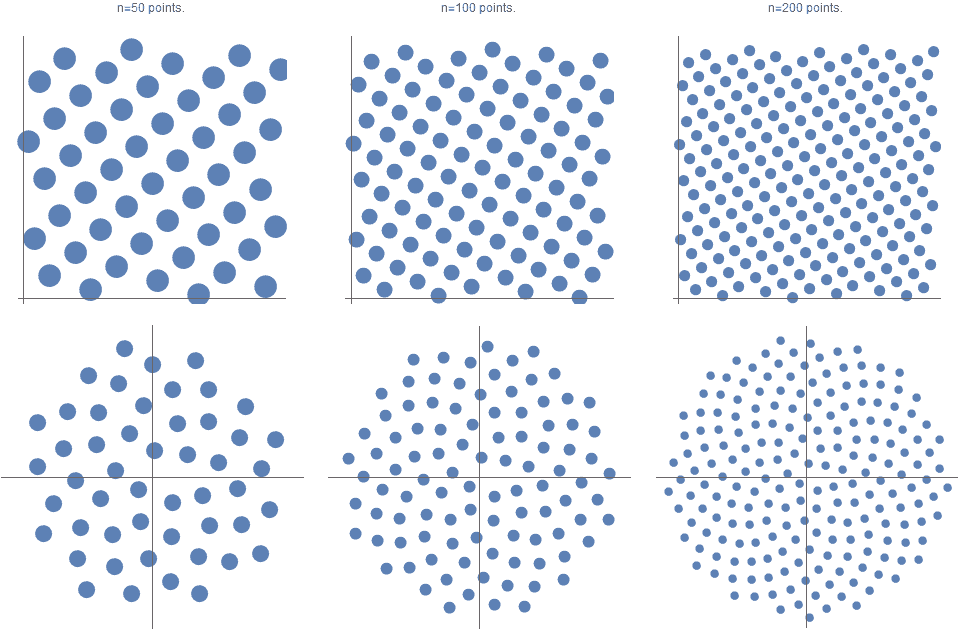
\includegraphics[width=\textwidth]{images/1.png}
    \caption{Примеры сеток Фибоначчи}
\end{figure}

\newpage

Аналогичным образом эти множества точек можно перенести из единичного квадрата $[0, 1]^2$ на сферу при помощи цилиндрической равновеликой проекции:

\begin{displaymath}
	(x,y) \rightarrow (\theta, \phi) : \quad \left( \cos^{-1}(2x-1) - \frac{\pi}{2}, 2\pi y \right),
\end{displaymath}

\begin{displaymath}
	(\theta,\phi) \rightarrow (x,y,z) : \quad \left (\cos\theta \cos\phi, \cos \theta \sin \phi, \sin \theta \right).
\end{displaymath}

Вот базовая реализация этого в Python:

\begin{lstlisting}[language=Python, numbers=left, xleftmargin=6mm]
from numpy import arange, pi, sin, cos, arccos
n = 50
i = arange(0, n, dtype=float) + 0.5
phi = arccos(1 - 2*i/n)
goldenRatio = (1 + 5**0.5)/2
theta = 2 pi * i / goldenRatio
x = cos(theta) * sin(phi)
y = sin(theta) * sin(phi)
z = cos(phi);
\end{lstlisting}

Даже несмотря на то, что сферические множества Фибоначчи глобально не являются наилучшим распределением сэмплов на сфере (потому что их решения не совпадают с решениями для платоновых тел при $n=4,6,8,12,20$), они обладают превосходными свойствами сэмплирования и очень легки в построении по сравнению с другими, более сложными схемами сферического сэмплирования.

Так как перенос из единичного квадрата на поверхность сферы выполняется проекцией с сохранением площади, можно ожидать, что если исходные точки распределены равномерно, то они также будут достаточно хорошо распределены и на поверхности сферы. Однако это не означает, что распределение будет доказуемо оптимальным.

Такой перенос страдает от двух различных, но взаимосвязанных проблем.

Во-первых, это наложение выполняется с сохранением площади, а не расстояния. Учитывая то, что в нашем случае условием является максимизация минимального попарного расстояния между точками, то такие условия и взаимосвязи необязательно будут выполняться после проецирования.

Вторую проблему сложнее всего решить с точки зрения практики: наложение имеет на каждом полюсе две вырожденные точки. Рассмотрим две точки, находящиеся очень близко к полюсу, но отличающиеся на 180 градусов по долготе. На единичном квадрате (и на цилиндрической проекции) они будут соответствовать двум очень далёким друг от друга точкам, однако при наложении на поверхность сферы они могут быть соединены очень малой дугой, проходящей через северный полюс. Из-за этой конкретной проблемы многие спиральные наложения оказываются недостаточно оптимальными.

\subsubsection*{Сетка 1}
\addcontentsline{toc}{subsubsection}{Сетка 1} % toc - table of contents

Более распространённая версия (особенно в компьютерных системах), создающая более хорошее значение $d^*=3.09$, имеет вид:

\begin{displaymath}
	t_i = \left( \frac{i + 0.5}{N}, \frac{i}{\phi} \right),
	\qquad
	0 \leq i \leq N-1.
	\tag{2}
\end{displaymath}

Она располагает точки в средних точках интервалах (по правилу средней точки в квадратной формуле Гаусса), поэтому для $n=100$, значения первой координаты будут такими:

\begin{displaymath}
	\{
		\frac{0.5}{100},
		\frac{1.5}{100},
		\frac{2.5}{100},
		\ldots,
		\frac{97.5}{100},
		\frac{98.5}{100},
		\frac{99.5}{100}
	\}.
\end{displaymath}

\subsubsection*{Сетка 2}
\addcontentsline{toc}{subsubsection}{Сетка 2} % toc - table of contents

Ключевым моментом для дальнейшего улучшения уравнения 2, является осознание того, что $d^*_N$ всегда соответствует расстоянию между точками $t_0$ и $t_3$, которые находятся на полюсах. То есть для улучшения $d_N$ точки рядом с полюсами должны быть разнесены ещё дальше.

Если мы определим следующее распределение:

\begin{displaymath}
	t_i = \left( \frac{i + \varepsilon}{N - 1 + 2 \varepsilon}, \frac{i}{\phi} \right),
	\qquad
	0 \leq i \leq N-1,
\end{displaymath}

\noindent $d^*_N$ — кривые для различных значений. $\varepsilon=0$ (синяя); $\varepsilon=\dfrac{1}{2}$ (оранжевая); $\varepsilon=\dfrac{3}{2}$ (зелёная); и $\varepsilon=\dfrac{5}{2}$ (красная). Можно увидеть, что $\varepsilon = \dfrac{5}{2}$ даёт результаты ближе к асимптотическим результатам. То есть при $N>20$ следующее простое выражение генерирует значительно более хорошие результаты $d^* = 3.29$ по сравнению с канонической сферической сеткой Фибоначчи:

\begin{displaymath}
	t_i = \left( \frac{i + 1.5}{N + 3}, \frac{i}{\phi} \right),
	\qquad
	0 \leq i \leq N-1.
	\tag{3}
\end{displaymath}

То есть при $N=100$ значения первой координаты будут равны:

\begin{displaymath}
	\{
		\frac{1.5}{103},
		\frac{2.5}{103},
		\frac{3.5}{103},
		\ldots,
		\frac{98.5}{103},
		\frac{99.5}{103},
		\frac{100.5}{103}
	\}.
\end{displaymath}

\begin{figure}[H]
    \centering
    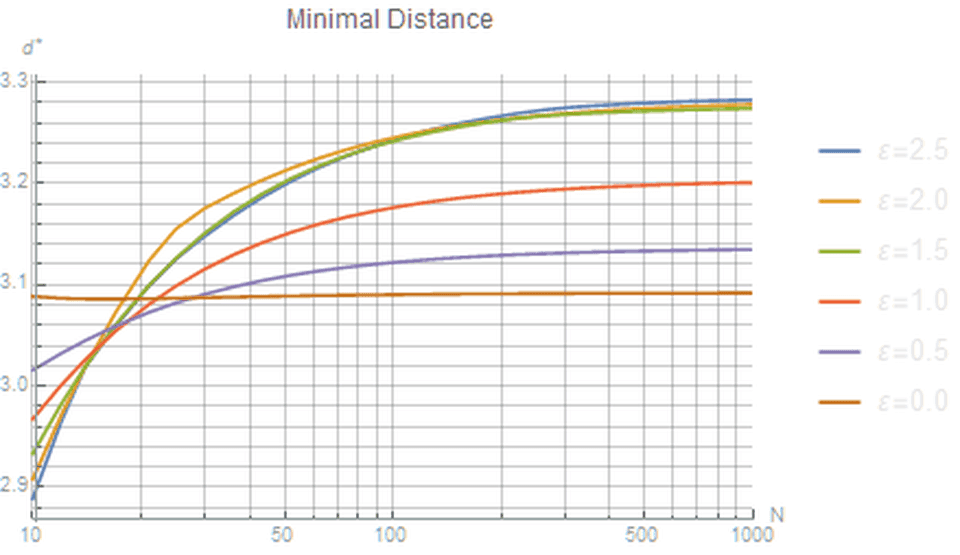
\includegraphics[width=\textwidth]{images/2.png}
    \caption{Различные значения $d_N^*$ при разных значениях $\epsilon$. Чем больше значение, тем оптимальнее конфигурации. Мы видим, что $\epsilon \simeq 2.5$ обеспечивает решение, близкое к оптимальному.}
\end{figure}

\subsubsection*{Сетка 3}
\addcontentsline{toc}{subsubsection}{Сетка 3} % toc - table of contents

Как сказано выше, одна из самых серьёзных проблем равномерного распределения точек на сфере заключается в том, что оптимальность распределения критически зависит от используемой целевой функции. Оказывается. что локальные величины наподобие $d_N^*$ иногда почти «не прощают ошибок» — единственная точка в недостаточно оптимальной позиции может катастрофически снизить оценку всего распределения точек.

В нашем случае вне зависимости от величины $N$ значение $D_N^*$ обычно определяется четырьмя точками, наиболее близкими к каждому из полюсов, особенно $t_0$ и $t_3$. Однако об этой сетке также известно то, что наибольший многоугольник Вороного находится на полюсе. Таким образом, пытаясь максимизировать $d_N$ разделением изначальных полярных точек в ряду, мы на самом деле ещё больше увеличиваем пустоту на полюсе! Поэтому мы представили альтернативу сетке 2, которая в общем случае более предпочтительна, потому что она не демонстрирует такой большой пустоты рядом с полюсами.

Она почти идентична сетке 2, но имеет два отличия. Во-первых, она использует $\varepsilon = \dfrac{11}{2}$ при $1 \leq i \leq N-2$. Во-вторых, кроме этих $N-2$ точек первая и последняя точки располагаются на каждом из полюсов.

То есть:

\begin{displaymath}
	t_0 = (0, 0),
	\qquad
	t_{N-1} = (1, 0),
	\qquad
	t_i = \left( \frac{i + 3.5}{N + 6}, \frac{i}{\phi} \right),
	\qquad
	0 \leq i \leq N-1.
	\tag{3}
\end{displaymath}

Удивительное свойство этого метода построения заключается в том, что несмотря на то, что его создание было мотивировано желанием минимизировать пустоты на полюсах, он на самом деле имеет наилучшее среди всех методов значение $d_N$ и $d^*$ с $d^* = 3.31$.

То есть при $N=100$ значения первой координаты будут такими:

\begin{displaymath}
	\{
		0,
		\frac{3.5}{106},
		\frac{4.5}{106},
		\frac{5.5}{106},
		\ldots,
		\frac{99.5}{106},
		\frac{100.5}{106},
		\frac{101.5}{106},
		1
	\}.
\end{displaymath}

\begin{figure}[H]
    \centering
    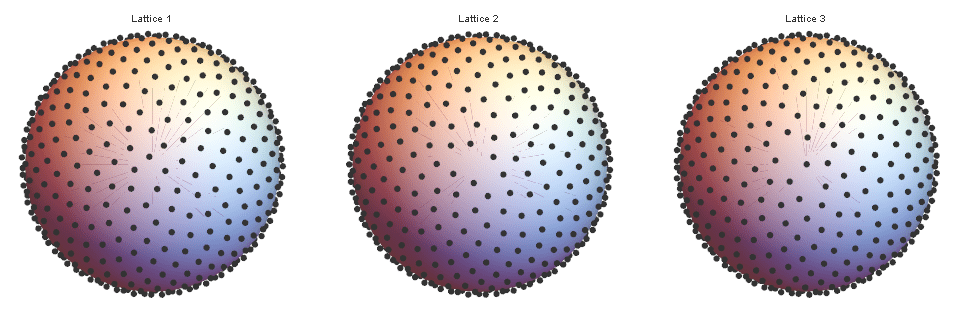
\includegraphics[width=\textwidth]{images/3.png}
    \caption{Различные конфигурации сеток. Каноническая сетка Фибоначчи слева. Заметьте, что несмотря на то, что у средней сетки $d_N^*$ улучшено, на полюсе у неё есть заметная пустота. Сетка 3 не имеет пустоты на полюсе и обладает наилучшим значением $d_N^*$.}
\end{figure}

\subsection{Сравнение}

При больших значениях $N$ это значение $d^*$ чрезвычайно хорошо сравнимо с другими методами, например, геодезическими куполами, которые основаны на триангулированных проекциях с граней платоновых тел на поверхность сферы. Неудивительно что самые качественные геодезические купола построены на основе икосаэдра или додекаэдра.

\begin{table}[H]
\caption{Основанные на икосаэдре геодезические купола при различных значениях $N$.}
\begin{center}
\begin{tabular}{ |c|c|c|c|c|c|c|c|c|c|c| } 
\hline
N & 12 & 42 & 92 & 162 & 252 & 362 & 492 & 642 & 812 & 1002 \\
\hline
$d^*$ & 3.64 & 3.54 & 3.34 & 3.22 & 3.15 & 3.09 & 3.06 & 3.03 & 3.00 & 2.99 \\
\hline
\end{tabular}
\end{center}
\end{table}

\begin{table}[H]
\caption{Основанные на додекаэдре геодезические купола при различных значениях $N$.}
\begin{center}
\begin{tabular}{ |c|c|c|c|c|c|c|c| } 
\hline
N & 20 & 32 & 122 & 272 & 482 & 752 & 1082 \\
\hline
$d^*$ & 3.19 & 3.63 & 3.16 & 2.99 & 2.90 & 2.84 & 2.81 \\
\hline
\end{tabular}
\end{center}
\end{table}

Кроме того, усечённый икосаэдр, соответствующий форме фуллерена $C_{60}$, имеет всего лишь $d^* = 3.125$.

То есть при $N>100$ сетки на основе уравнения 3 лучше любых геодезических многограннико.

По данным из первого источника в представленном ниже списке справочной литературы, некоторые из современных методов, которые обычно сложны и требуют рекурсивного и/или динамического программирования, имеют следующие показатели.

\begin{table}[H]
\caption{Показатель $d^*$  для разлилчных современных методов распределения точек на сфере}
\begin{center}
\begin{tabular}{ |c|c| } 
\hline
Метод &  $d^*$ \\
\hline
Lattice 1 & 3.09 \\
\hline
Max Determinant & 3.19 \\
\hline
Lattice 2 & 3.28 \\
\hline
Lattice 3 & 3.31 \\
\hline
Zonal Equal Area & 3.32 \\
\hline
Coulomb & 3.37 \\
\hline
Log Energy & 3.37 \\
\hline
\end{tabular}
\end{center}
\end{table}

\subsection{Вывод из раздела 1}

Сетка 3, созданная по уравнению 3, является модификацией канонической сетки Фибоначчи, обеспечивающей гораздо более качественную упаковку распределения точек. То есть:

\begin{displaymath}
	t_0 = (0, 0),
	\qquad
	t_{N-1} = (0, 1),
	\qquad
	t_i = \left( \frac{i + 6}{N + 11}, \frac{i}{\phi} \right),
	\qquad
	0 \leq i \leq N-1.
	\tag{3}
\end{displaymath}

\newpage

\section{Оптимизация выпуклой оболочки (сетки Делоне)}

В предыдущем разделе мы оптимизировали распределение по $d^*_N$, однако эти модификации ухудшают другие показатели, например объём выпуклой оболочки (сетки Делоне). В этом разделе рассказывается, как равномерно распределить точки на сфере таким образом чтобы оптимизировать (максимизировать) такой более глобальный показатель, как объём выпуклой оболочки.

Обозначим $\epsilon_N$ как выпуклую оболочку $N$ точек:

\begin{displaymath}
	\epsilon_N = N \left( \frac{4 \pi}{3} - Vol(C_N) \right),
\end{displaymath}

\noindent сюда включён фактор нормализации $N$, потому что абсолютное расхождение снижается со скоростью $\frac{1}{N}$.

Поведение $\varepsilon_N$ при различных $N$ можно увидеть на рисунке 4 (синяя линия).

Для снижения рассогласованности объёмов необходимо заметить, что несмотря на использование $\phi$, из логичности золотого сечения при $N \rightarrow \infty$ необязательно следует, что оно является наилучшим значением для конечного $N$. Говоря по-научному, можно сказать, что нужно учесть влияние коррекции конечности членов.

Давайте обобщим уравнение 1 следующим образом:

\begin{displaymath}
	t_i = \left( \frac{i+1/2}{N}, \frac{i}{g(N)} \right), \qquad 0 \leq i \leq N-1,
	\tag{4}
\end{displaymath}

\noindent где определим $g(n)$ как:

\begin{displaymath}
	g(n) =
		\begin{cases}
			3-\phi, & \text{если $k$ чётное} \\
			\phi, & \text{если $k$ нечетное}
		\end{cases},
	\tag{5}
\end{displaymath}

\begin{displaymath}
	k =
		\left\lfloor
			\log_{\phi}(\frac{n}{1.5})
		\right\rfloor
	  =
		\left\lfloor
			\frac{\ln (n/1.5)}{\ln \phi }
		\right\rfloor,
\end{displaymath}

\noindent где $\lfloor x \rfloor$ — функция округления до ближайшего целого в меньшую сторону.

Причина этого заключается в следующем факте: все числа $x$, удовлетворяющие особому преобразованию Мёбиуса, исходя из иррациональности эквивалентны $\phi$:

\begin{displaymath}
	x = \frac{a\phi+b}{c\phi+d}, \qquad \textrm{для всех } a,b,c,d, |ad-bc|=1.
\end{displaymath}

Следовательно, причина того, что $\phi$ и $3-\phi$ так хорошо подходят друг другу, заключается в том, что:

\begin{displaymath}
	\frac{1}{\phi} = \frac{\phi+1}{2\phi+1}, \qquad \frac{1}{3-\phi}= \frac{2\phi+1}{1\phi+1}.
\end{displaymath}

\begin{figure}[H]
    \centering
    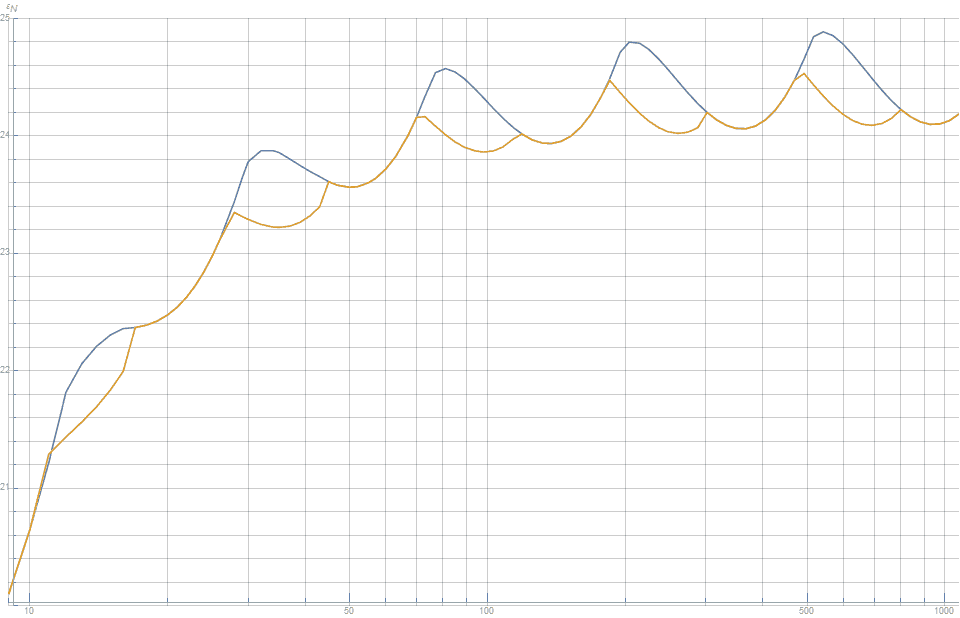
\includegraphics[width=\textwidth]{images/4.png}
    \caption{Рассогласованность между объёмом выпуклой оболочки из точек и объёмом единичной сферы. Учтите, что чем она меньше, тем лучше. Рисунок показывает, что гибридная модель (оранжевая линия), основанная на $\phi$ и $3-\phi$, обеспечивает более качественное распределение точек, чем каноническая сетка Фибоначчи (голубая линия).}
\end{figure}

Для оставшейся половины мы сначала определим вспомогательный ряд $A_N$, являющийся разновидностью ряда Фибоначчи:

\begin{displaymath}
	A_1 =1, A_2 = 4, A_{n+2}= A_{n+1}+A_n \textrm{ для } n = 1,2,3, \ldots,
\end{displaymath}

\noindent то есть:

\begin{displaymath}
	A_N = 1,4,5,9,14,23,37,60,97,157,254,411, \ldots.
\end{displaymath}

\newpage

Все дроби этого ряда имеют изящные непрерывные дроби, а в пределе сходятся к $\phi$. Например:

\begin{displaymath}
	\frac{t_5}{t_4} = 1 + \cfrac{1}{1 + \cfrac{1}{1 + \cfrac{1}{ 1 + \cfrac{1}{4}}}}.
\end{displaymath}

Теперь мы можем полностью обобщить $g(n)$ следующим образом:

\begin{displaymath}
	g(N) =
		\begin{cases}
			3-\phi, & \text{если $k$ четное} \\
			\dfrac{A_{j+1}}{A_j} , & \text{если $k$ нечетное, $j=\dfrac{k+7}{2}$}
 		\end{cases}.
	\tag{6}
\end{displaymath}

\begin{table}[H]
\caption{Значения $g(N)$ для различных $N$.}
\begin{center}
\begin{tabular}{ |c|c|c|c|c|c|c|c|c|c| } 
\hline
\rule[-1.5ex]{0pt}{4.5ex} N & 4-6 & 7-10 & 11-16 & 17-26 & 27-43 & 44-70 & 71-114 & 115-184 & 185-300 \\
\hline
\rule[-3ex]{0pt}{7.5ex} g(n) & $3-\phi$ & $\dfrac{23}{14}$ & $3-\phi$ & $\dfrac{37}{23}$ & $3-\phi$ & $\dfrac{60}{37}$ & $3-\phi$ & $\dfrac{97}{60}$ & $3-\phi$ \\
\hline
\end{tabular}
\end{center}
\end{table}

Из рисунка 4 видно, что относительно объёма выпуклой оболочки это новое распределение лучше, чем каноническая сетка для всех значений $n$.

\begin{figure}[H]
    \centering
    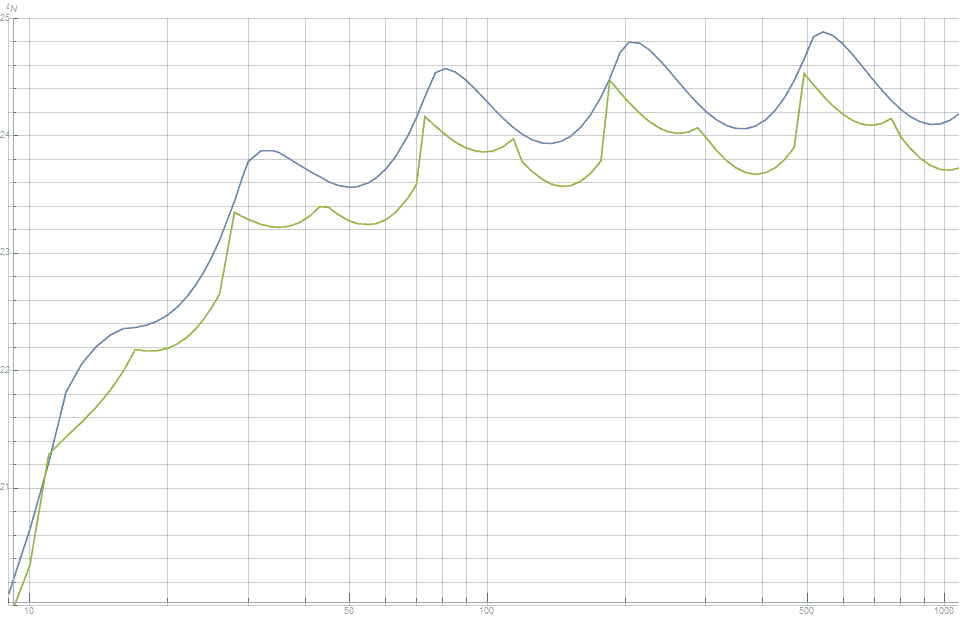
\includegraphics[width=\textwidth]{images/5.png}
    \caption{Рассогласование между объёмом выпуклой оболочки и объёмом единичной сферы. Чем меньше значения, тем лучше. Это говорит нам, что предлагаемый новый метод (зелёная линия) постоянно обеспечивает лучшее по сравнению с канонической сеткой Фибоначчи (синяя линия) распределение.}
\end{figure}

\begin{figure}[H]
    \centering
    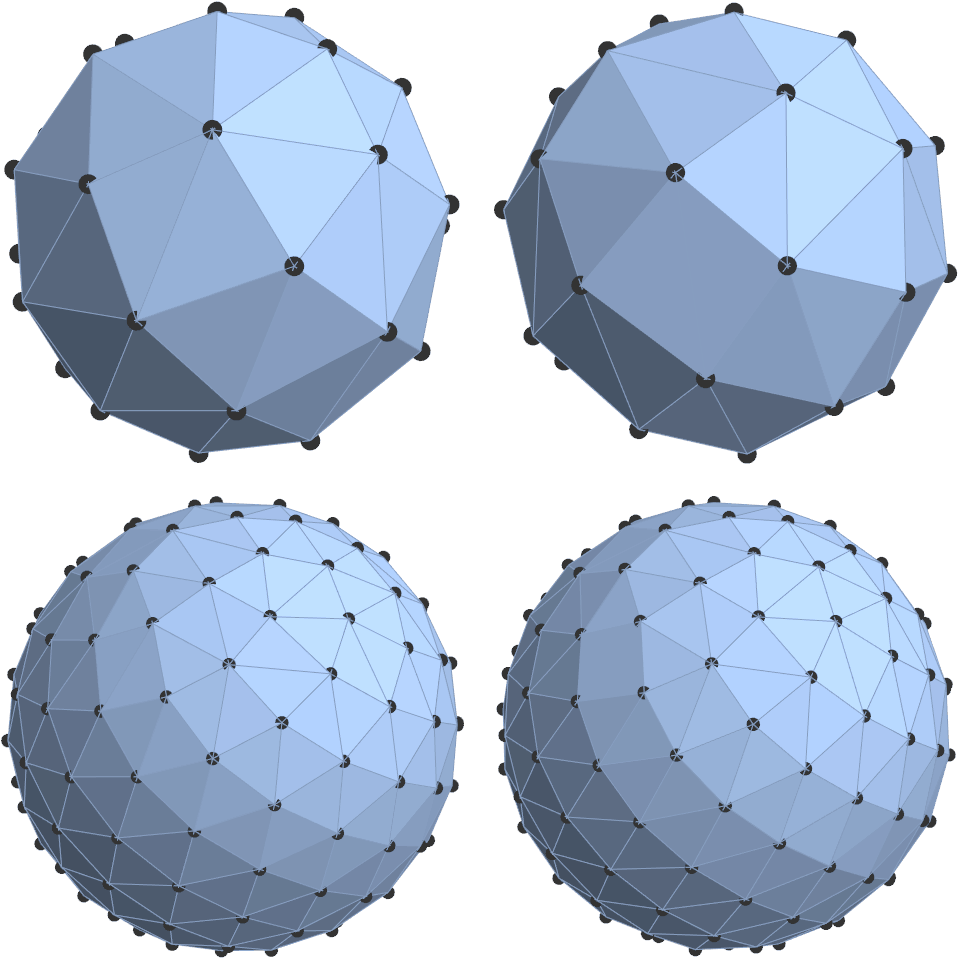
\includegraphics[width=\textwidth]{images/6.png}
    \caption{Наглядное сравнение канонической сетки (слева) с новой модифицированной сеткой (справа) при n=35 и n=150. Визуально различия почти незаметны. Однако в условиях, требующих максимальной эффективности, модифицированная версия (справа) обеспечивает небольшое, но поддающееся количественному измерению улучшению и в объёме, и в площади поверхности выпуклой оболочки.}
\end{figure}

Любопытно, что это распределение также незначительно, но неуклонно снижает рассогласование между площадью поверхности выпуклой оболочки и площадью поверхности единичной сферы. Это показано на рисунке 6.

\begin{figure}[H]
    \centering
    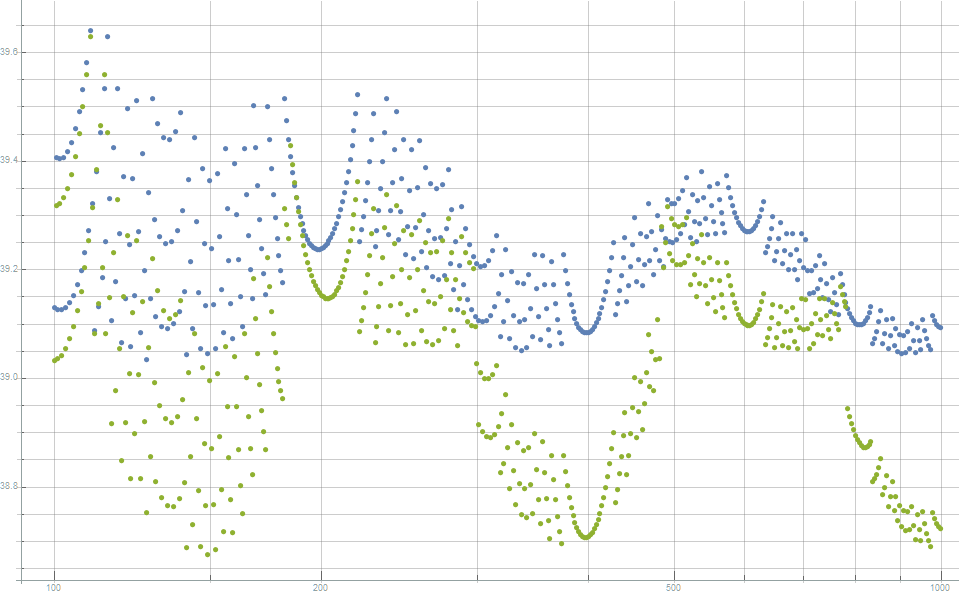
\includegraphics[width=\textwidth]{images/7.png}
    \caption{Нормализованное рассогласование площадей между площадью поверхности выпуклой оболочки (сетки Делоне) и площадью поверхности единичной сферы. Чем ниже значения, тем лучше. Это показывает, что предложенная новая модификация (зелёные точки) демонстрирует небольшое, но постоянное снижение разности площадей поверхностей по сравнению с канонической сеткой Фибоначчи (синие точки)}
\end{figure}

\subsection{Вывод из раздела 2}

Сетка, соответствующая уравнению 6, является модификацией канонической сетки Фибоначчи, создающей значительно лучшее распределение точек, исходя из объёма и площади поверхности выпуклой оболочки (сетки Делоне).

\newpage

\section*{}
\addcontentsline{toc}{section}{Список литературы} % toc - table of contents

\bibliographystyle{gost705}  % gost705-2008
\nocite{*}  % включение в список литературы всех записей из базы данных
\bibliography{sources}         % bib-files

\end{document}